\textcolor{red}{comparer les perfs des intersections volumétriques avec les intersections de Mesh}

Résultat de l'implémentation des maillages d'une sphère de subdivision (subdivision dyadique), d'un tore, d'une capsule et d'un cylindre:

\begin{figure}[h!]
	\adjustbox{center}{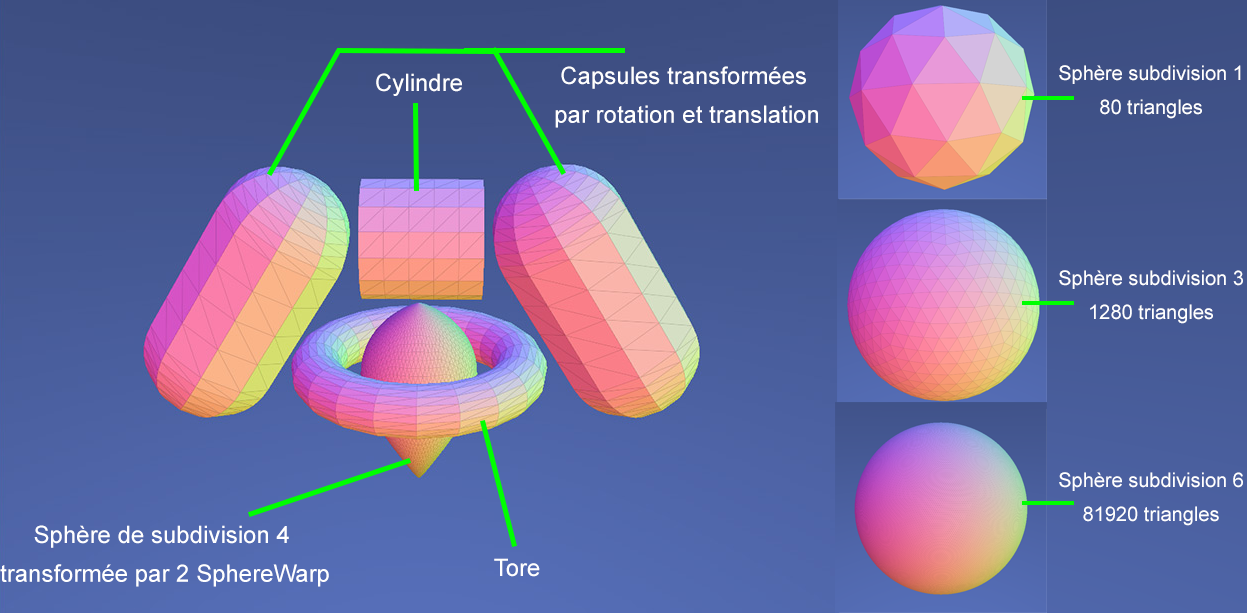
\includegraphics[width=1.2\textwidth]{Captures/IllustrationAnnotations.png}}

	\caption{Union de maillages grâce à Mesh::Merge}
\end{figure}
\FloatBarrier
